\documentclass[tikz,border=2pt]{standalone}
\usepackage{amsmath,amssymb}
\usepackage{pgfplots}
\pgfplotsset{compat=1.18}

\begin{document}
% Conditional CDF of X given Y = y when X | Y = y ~ Unif(0, y): a ramp x/y on (0, y), one curve
% for each value of y; the conditional median is y/2.
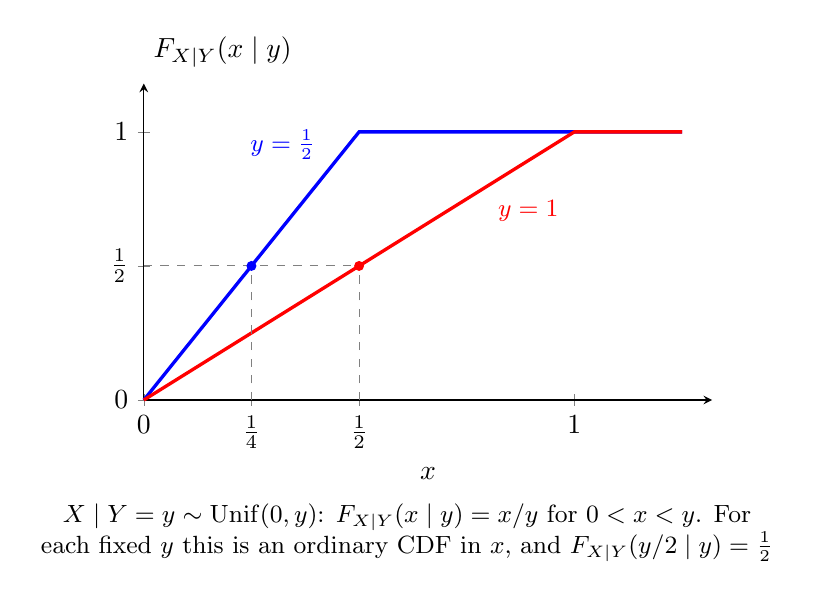
\begin{tikzpicture}
	\begin{axis}[
		axis lines=left, xmin=0, xmax=1.32, ymin=0, ymax=1.18,
		xtick={0,0.25,0.5,1}, xticklabels={$0$,$\tfrac14$,$\tfrac12$,$1$}, ytick={0,0.5,1}, yticklabels={$0$,$\tfrac12$,$1$},
		xlabel={$x$}, ylabel={$F_{X\mid Y}(x\mid y)$}, ylabel style={rotate=-90, anchor=south west, at={(axis description cs:0,1.02)}},
		width=8.8cm, height=5.6cm, clip=false
		]
		\addplot[blue, very thick] coordinates {(0,0) (0.5,1) (1.25,1)};
		\addplot[red, very thick] coordinates {(0,0) (1,1) (1.25,1)};
		\draw[gray, dashed] (axis cs:0,0.5) -- (axis cs:0.5,0.5);
		\draw[gray, dashed] (axis cs:0.25,0) -- (axis cs:0.25,0.5);
		\draw[gray, dashed] (axis cs:0.5,0) -- (axis cs:0.5,0.5);
		\fill[blue] (axis cs:0.25,0.5) circle (1.8pt);
		\fill[red] (axis cs:0.5,0.5) circle (1.8pt);
		\node[blue, anchor=south east, font=\small] at (axis cs:0.42,0.86) {$y=\tfrac12$};
		\node[red, anchor=north west, font=\small] at (axis cs:0.8,0.78) {$y=1$};
	\end{axis}
	\node[anchor=north, font=\small, align=flush center, text width=9.4cm] at ([yshift=-2pt]current axis.outer south) {$X\mid Y=y\sim\operatorname{Unif}(0,y)$: $F_{X\mid Y}(x\mid y)=x/y$ for $0<x<y$. For each fixed $y$ this is an ordinary CDF in $x$, and $F_{X\mid Y}(y/2\mid y)=\tfrac12$};
\end{tikzpicture}
\end{document}
